\documentclass[9pt]{beamer}
\usetheme{cmepda}

\usepackage[utf8]{inputenc}
\usepackage[T1]{fontenc}


\title{Python Basics (1/2)}
\subtitle{Computing Methods for Experimental Physics and Data Analysis}
\date{Compiled on \today}
\author{L. Baldini}
\institute[UNIPI and INFN]{Universit\`a and INFN--Pisa}
\email{luca.baldini@pi.infn.it}


\begin{document}


\titleframe

\begin{frame}
  \frametitle{Python 3 vs. Python 2}
  \begin{itemize}
  \item You might have heard about the Python 2 vs. Python 3 diatribe
  \item What's new in Python 3?
    \begin{itemize}
    \item print() is a function (vs. a statement)
    \item Integer division returns a float (hurray!)
    \item But really, \alert{the big change is the implementation of
      unicode support}
      \begin{itemize}
      \item Although you probably don't care that much if you are a data
        scientist
      \end{itemize}
    \end{itemize}
  \item Python 3 is the future!
    \begin{itemize}
    \item Python 2 EOL (End Of Life) \emph{was} January 1, 2020
    \item Hundreds of features introduced in Python 3 and not backported to
      Python 2
    \item All third-party modules worth mentioning support both Python 2 and
      Python 3, these days
    \end{itemize}
  \item \alert{One-line summary: we shall be using Python 3}
  \end{itemize}
\end{frame}


\begin{frame}[fragile]
  \frametitle{The zen of Python}
  \framesubtitle{See PEP 20, \url{https://www.python.org/dev/peps/pep-0020/}}
  \begin{Verbatim}
[lbaldini@nbbaldini slides]$ python
Python 3.7.4 (default, Jul  9 2019, 16:32:37)
[GCC 9.1.1 20190503 (Red Hat 9.1.1-1)] on linux
Type "help", "copyright", "credits" or "license" for more information.
>>> import this
The Zen of Python, by Tim Peters

Beautiful is better than ugly.
Explicit is better than implicit.
Simple is better than complex.
Complex is better than complicated.
Flat is better than nested.
Sparse is better than dense.
Readability counts.
Special cases aren't special enough to break the rules.
Although practicality beats purity.
Errors should never pass silently.
Unless explicitly silenced.
In the face of ambiguity, refuse the temptation to guess.
There should be one-- and preferably only one --obvious way to do it.
Although that way may not be obvious at first unless you're Dutch.
Now is better than never.
Although never is often better than *right* now.
If the implementation is hard to explain, it's a bad idea.
If the implementation is easy to explain, it may be a good idea.
Namespaces are one honking great idea -- let's do more of those!
  \end{Verbatim}
\end{frame}


\begin{frame}
  \frametitle{Coding conventions?}
  \framesubtitle{\url{https://www.python.org/dev/peps/pep-0008/}}
  \begin{itemize}
  \item \emph{Coding conventions} are guidelines about how to write code
    \begin{itemize}
    \item Different for different languages
    \item i.e., you are encouraged to stick to them, but your code will
      happily run if you don't
    \end{itemize}
  \item \alert{Then why should I care?}
  \item Code is read much more often than it is written
    \begin{itemize}
    \item Readability counts (the zen of Python)
    \end{itemize}
  \item One-line summary: \alert{think about it but don't be obsessed by it}
  \item The bible of coding conventions for Python is \url{https://www.python.org/dev/peps/pep-0008/}
  \item There are automatic tools out there to help you
    \begin{itemize}
      \item https://www.pylint.org/
      \item https://pypi.org/project/pyflakes/
      \item http://mypy-lang.org/
      \item https://github.com/PyCQA/pycodestyle
    \end{itemize}
  \end{itemize}
\end{frame}


\begin{frame}
  \frametitle{Variables and basic types}
  \begin{Verbatim}[label=\makebox{\url{https://github.com/lucabaldini/cmepda/tree/master/slides/latex/snippets/basic\_types.py}},commandchars=\\\{\}]
\PY{n}{i} \PY{o}{=} \PY{l+m+mi}{3}
\PY{n}{x} \PY{o}{=} \PY{l+m+mf}{3.0}
\PY{k}{print}\PY{p}{(}\PY{n}{i}\PY{p}{,} \PY{n+nb}{type}\PY{p}{(}\PY{n}{i}\PY{p}{)}\PY{p}{)}
\PY{k}{print}\PY{p}{(}\PY{n}{x}\PY{p}{,} \PY{n+nb}{type}\PY{p}{(}\PY{n}{x}\PY{p}{)}\PY{p}{)}

\PY{n}{s} \PY{o}{=} \PY{l+s+s1}{\PYZsq{}}\PY{l+s+s1}{Hi there!}\PY{l+s+s1}{\PYZsq{}}
\PY{k}{print}\PY{p}{(}\PY{n}{s}\PY{p}{,} \PY{n+nb}{type}\PY{p}{(}\PY{n}{s}\PY{p}{)}\PY{p}{)}

\PY{n}{l} \PY{o}{=} \PY{p}{[}\PY{l+m+mi}{1}\PY{p}{,} \PY{l+m+mi}{2}\PY{p}{,} \PY{l+s+s1}{\PYZsq{}}\PY{l+s+s1}{a string}\PY{l+s+s1}{\PYZsq{}}\PY{p}{]}
\PY{k}{print}\PY{p}{(}\PY{n}{l}\PY{p}{,} \PY{n+nb}{type}\PY{p}{(}\PY{n}{l}\PY{p}{)}\PY{p}{,} \PY{n}{l}\PY{p}{[}\PY{l+m+mi}{0}\PY{p}{]}\PY{p}{)}

\PY{n}{t} \PY{o}{=} \PY{p}{(}\PY{l+m+mi}{1}\PY{p}{,} \PY{l+m+mi}{2}\PY{p}{,} \PY{l+s+s1}{\PYZsq{}}\PY{l+s+s1}{a string}\PY{l+s+s1}{\PYZsq{}}\PY{p}{)}
\PY{k}{print}\PY{p}{(}\PY{n}{t}\PY{p}{,} \PY{n+nb}{type}\PY{p}{(}\PY{n}{t}\PY{p}{)}\PY{p}{,} \PY{n}{t}\PY{p}{[}\PY{l+m+mi}{0}\PY{p}{]}\PY{p}{)}

\PY{n}{d} \PY{o}{=} \PY{p}{\PYZob{}}\PY{l+s+s1}{\PYZsq{}}\PY{l+s+s1}{key1}\PY{l+s+s1}{\PYZsq{}}\PY{p}{:} \PY{l+m+mi}{1}\PY{p}{,} \PY{l+s+s1}{\PYZsq{}}\PY{l+s+s1}{key2}\PY{l+s+s1}{\PYZsq{}}\PY{p}{:} \PY{l+m+mi}{2}\PY{p}{\PYZcb{}}
\PY{k}{print}\PY{p}{(}\PY{n}{d}\PY{p}{,} \PY{n+nb}{type}\PY{p}{(}\PY{n}{d}\PY{p}{)}\PY{p}{,} \PY{n}{d}\PY{p}{[}\PY{l+s+s1}{\PYZsq{}}\PY{l+s+s1}{key1}\PY{l+s+s1}{\PYZsq{}}\PY{p}{]}\PY{p}{)}

[Output]
3 <class 'int'>
3.0 <class 'float'>
Hi there! <class 'str'>
[1, 2, 'a string'] <class 'list'> 1
(1, 2, 'a string') <class 'tuple'> 1
{'key1': 1, 'key2': 2} <class 'dict'> 1
\end{Verbatim}
\end{frame}


\begin{frame}
  \frametitle{Digression: string formatting}
  \begin{Verbatim}[label=\makebox{\url{https://github.com/lucabaldini/cmepda/tree/master/slides/latex/snippets/string\_formatting.py}},commandchars=\\\{\}]
\PY{n}{name} \PY{o}{=} \PY{l+s+s1}{\PYZsq{}}\PY{l+s+s1}{Luca}\PY{l+s+s1}{\PYZsq{}}
\PY{n}{age} \PY{o}{=} \PY{l+m+mi}{42}

\PY{c+c1}{\PYZsh{} The ugly way.}
\PY{k}{print}\PY{p}{(}\PY{l+s+s1}{\PYZsq{}}\PY{l+s+s1}{My name is }\PY{l+s+s1}{\PYZsq{}} \PY{o}{+} \PY{n}{name} \PY{o}{+} \PY{l+s+s1}{\PYZsq{}}\PY{l+s+s1}{ I am }\PY{l+s+s1}{\PYZsq{}} \PY{o}{+} \PY{n+nb}{str}\PY{p}{(}\PY{n}{age}\PY{p}{)} \PY{o}{+} \PY{l+s+s1}{\PYZsq{}}\PY{l+s+s1}{ year(s) old.}\PY{l+s+s1}{\PYZsq{}}\PY{p}{)}

\PY{c+c1}{\PYZsh{} The old way (\PYZpc{} operator)}
\PY{k}{print}\PY{p}{(}\PY{l+s+s1}{\PYZsq{}}\PY{l+s+s1}{My name is }\PY{l+s+si}{\PYZpc{}s}\PY{l+s+s1}{ I am }\PY{l+s+si}{\PYZpc{}d}\PY{l+s+s1}{ year(s) old.}\PY{l+s+s1}{\PYZsq{}} \PY{o}{\PYZpc{}} \PY{p}{(}\PY{n}{name}\PY{p}{,} \PY{n}{age}\PY{p}{)}\PY{p}{)}

\PY{c+c1}{\PYZsh{} The new way (.format)}
\PY{c+c1}{\PYZsh{} This is actually *much* more powerful and flexible than implied here.}
\PY{k}{print}\PY{p}{(}\PY{l+s+s1}{\PYZsq{}}\PY{l+s+s1}{My name is \PYZob{}\PYZcb{} I am \PYZob{}\PYZcb{} year(s) old.}\PY{l+s+s1}{\PYZsq{}}\PY{o}{.}\PY{n}{format}\PY{p}{(}\PY{n}{name}\PY{p}{,} \PY{n}{age}\PY{p}{)}\PY{p}{)}

\PY{c+c1}{\PYZsh{} The newer way\PYZhy{}\PYZhy{}\PYZhy{}new in Python 3.6. This is awesome!}
\PY{k}{print}\PY{p}{(}\PY{n}{f}\PY{l+s+s1}{\PYZsq{}}\PY{l+s+s1}{My name is \PYZob{}name\PYZcb{} I am \PYZob{}age\PYZcb{} year(s) old.}\PY{l+s+s1}{\PYZsq{}}\PY{p}{)}

[Output]
My name is Luca I am 42 year(s) old.
My name is Luca I am 42 year(s) old.
My name is Luca I am 42 year(s) old.
My name is Luca I am 42 year(s) old.
\end{Verbatim}
  \begin{itemize}
  \item String formatting in a nutshell:
    \begin{itemize}
    \item Never add strings
    \item Try and avoid using the \texttt{\%} operator
    \item Go for format(), and use f-strings if you can
    \end{itemize}
  \end{itemize}
\end{frame}


\begin{frame}
  \frametitle{Defining functions}
  \framesubtitle{\url{https://en.wikipedia.org/wiki/Don\%27t_repeat_yourself}}
  \begin{itemize}
  \item\alert{DRY (Don't Repeat Yourself) is better than WET (Write Every Time)}
  \end{itemize}

  \bigskip

  \begin{Verbatim}[label=\makebox{\url{https://github.com/lucabaldini/cmepda/tree/master/slides/latex/snippets/func1.py}},commandchars=\\\{\}]
\PY{k+kn}{import} \PY{n+nn}{math}

\PY{k}{def} \PY{n+nf}{square}\PY{p}{(}\PY{n}{x}\PY{p}{)}\PY{p}{:}
    \PY{l+s+sd}{\PYZdq{}\PYZdq{}\PYZdq{}Return the square of x.}
\PY{l+s+sd}{    \PYZdq{}\PYZdq{}\PYZdq{}}
    \PY{k}{return} \PY{n}{x} \PY{o}{*} \PY{n}{x}

\PY{k}{def} \PY{n+nf}{cartesian\PYZus{}to\PYZus{}polar}\PY{p}{(}\PY{n}{x}\PY{o}{=}\PY{l+m+mf}{1.}\PY{p}{,} \PY{n}{y}\PY{o}{=}\PY{l+m+mf}{1.}\PY{p}{)}\PY{p}{:}
    \PY{l+s+sd}{\PYZdq{}\PYZdq{}\PYZdq{}Convert cartesian to polar coordinates.}
\PY{l+s+sd}{    \PYZdq{}\PYZdq{}\PYZdq{}}
    \PY{n}{r} \PY{o}{=} \PY{n}{math}\PY{o}{.}\PY{n}{sqrt}\PY{p}{(}\PY{n}{x}\PY{o}{*}\PY{o}{*}\PY{l+m+mf}{2.} \PY{o}{+} \PY{n}{y}\PY{o}{*}\PY{o}{*}\PY{l+m+mf}{2.}\PY{p}{)}
    \PY{n}{phi} \PY{o}{=} \PY{n}{math}\PY{o}{.}\PY{n}{atan2}\PY{p}{(}\PY{n}{y}\PY{p}{,} \PY{n}{x}\PY{p}{)}
    \PY{k}{return} \PY{n}{r}\PY{p}{,} \PY{n}{phi}

\PY{k}{print}\PY{p}{(}\PY{n}{square}\PY{p}{(}\PY{l+m+mf}{2.}\PY{p}{)}\PY{p}{)}
\PY{k}{print}\PY{p}{(}\PY{n}{cartesian\PYZus{}to\PYZus{}polar}\PY{p}{(}\PY{l+m+mf}{0.}\PY{p}{,} \PY{l+m+mf}{1.}\PY{p}{)}\PY{p}{)}
\PY{k}{print}\PY{p}{(}\PY{n}{cartesian\PYZus{}to\PYZus{}polar}\PY{p}{(}\PY{p}{)}\PY{p}{)}

[Output]
4.0
(1.0, 1.5707963267948966)
(1.4142135623730951, 0.7853981633974483)
\end{Verbatim}
\end{frame}


\begin{frame}
  \frametitle{Variadic functions}
  \begin{itemize}
  \item Variadic functions accept a variable number of arguments
    \begin{itemize}
    \item More elegant than passing a list or a tuple of arguments
    \item How the heck is \emph{that} implemented?
    \end{itemize}
  \end{itemize}

  \bigskip

  \begin{Verbatim}[label=\makebox{\url{https://github.com/lucabaldini/cmepda/tree/master/slides/latex/snippets/func\_variadic1.py}},commandchars=\\\{\}]
\PY{k+kn}{import} \PY{n+nn}{os}

\PY{n}{p1} \PY{o}{=} \PY{n}{os}\PY{o}{.}\PY{n}{path}\PY{o}{.}\PY{n}{join}\PY{p}{(}\PY{l+s+s1}{\PYZsq{}}\PY{l+s+s1}{path}\PY{l+s+s1}{\PYZsq{}}\PY{p}{,} \PY{l+s+s1}{\PYZsq{}}\PY{l+s+s1}{to}\PY{l+s+s1}{\PYZsq{}}\PY{p}{,} \PY{l+s+s1}{\PYZsq{}}\PY{l+s+s1}{my}\PY{l+s+s1}{\PYZsq{}}\PY{p}{,} \PY{l+s+s1}{\PYZsq{}}\PY{l+s+s1}{file}\PY{l+s+s1}{\PYZsq{}}\PY{p}{)}
\PY{n}{p2} \PY{o}{=} \PY{n}{os}\PY{o}{.}\PY{n}{path}\PY{o}{.}\PY{n}{join}\PY{p}{(}\PY{l+s+s1}{\PYZsq{}}\PY{l+s+s1}{howdy}\PY{l+s+s1}{\PYZsq{}}\PY{p}{,} \PY{l+s+s1}{\PYZsq{}}\PY{l+s+s1}{partner}\PY{l+s+s1}{\PYZsq{}}\PY{p}{)}

\PY{k}{print}\PY{p}{(}\PY{n}{p1}\PY{p}{)}
\PY{k}{print}\PY{p}{(}\PY{n}{p2}\PY{p}{)}

\PY{n}{s1} \PY{o}{=} \PY{n+nb}{sum}\PY{p}{(}\PY{p}{[}\PY{l+m+mi}{1}\PY{p}{,} \PY{l+m+mi}{2}\PY{p}{]}\PY{p}{)}
\PY{n}{s2} \PY{o}{=} \PY{n+nb}{sum}\PY{p}{(}\PY{p}{[}\PY{l+m+mi}{1}\PY{p}{,} \PY{l+m+mi}{2}\PY{p}{,} \PY{l+m+mi}{3}\PY{p}{,} \PY{l+m+mi}{4}\PY{p}{,} \PY{l+m+mi}{5}\PY{p}{]}\PY{p}{)}

\PY{k}{print}\PY{p}{(}\PY{n}{s1}\PY{p}{)}
\PY{k}{print}\PY{p}{(}\PY{n}{s2}\PY{p}{)}

[Output]
path/to/my/file
howdy/partner
3
15
\end{Verbatim}
\end{frame}


\begin{frame}
  \frametitle{Arbitrary argument lists}
  \begin{Verbatim}[label=\makebox{\url{https://bitbucket.org/lbaldini/programming/src/tip/snippets/func\_variadic2.py}},commandchars=\\\{\}]
\PY{k+kn}{import} \PY{n+nn}{os}

\PY{k}{def} \PY{n+nf}{join1}\PY{p}{(}\PY{o}{*}\PY{n}{args}\PY{p}{)}\PY{p}{:}
    \PY{l+s+sd}{\PYZdq{}\PYZdq{}\PYZdq{}Horrible: do not use the + operator with strings in a loop.}
\PY{l+s+sd}{    \PYZdq{}\PYZdq{}\PYZdq{}}
    \PY{n}{out} \PY{o}{=} \PY{l+s+s1}{\PYZsq{}}\PY{l+s+s1}{\PYZsq{}}
    \PY{k}{for} \PY{n}{arg} \PY{o+ow}{in} \PY{n}{args}\PY{p}{:}
        \PY{n}{out} \PY{o}{+}\PY{o}{=} \PY{l+s+s1}{\PYZsq{}}\PY{l+s+si}{\PYZpc{}s}\PY{l+s+s1}{/}\PY{l+s+s1}{\PYZsq{}} \PY{o}{\PYZpc{}} \PY{n}{arg}
    \PY{k}{return} \PY{n}{out}\PY{o}{.}\PY{n}{rstrip}\PY{p}{(}\PY{l+s+s1}{\PYZsq{}}\PY{l+s+s1}{/}\PY{l+s+s1}{\PYZsq{}}\PY{p}{)}

\PY{k}{def} \PY{n+nf}{join2}\PY{p}{(}\PY{o}{*}\PY{n}{args}\PY{p}{)}\PY{p}{:}
    \PY{l+s+sd}{\PYZdq{}\PYZdq{}\PYZdq{}This a more sensible version\PYZhy{}\PYZhy{}\PYZhy{}and you get the idea of the *.}
\PY{l+s+sd}{    \PYZdq{}\PYZdq{}\PYZdq{}}
    \PY{k}{return} \PY{l+s+s1}{\PYZsq{}}\PY{l+s+s1}{/}\PY{l+s+s1}{\PYZsq{}}\PY{o}{.}\PY{n}{join}\PY{p}{(}\PY{n}{args}\PY{p}{)}

\PY{k}{def} \PY{n+nf}{join3}\PY{p}{(}\PY{o}{*}\PY{n}{args}\PY{p}{,} \PY{n}{sep}\PY{o}{=}\PY{n}{os}\PY{o}{.}\PY{n}{path}\PY{o}{.}\PY{n}{sep}\PY{p}{)}\PY{p}{:}
    \PY{l+s+sd}{\PYZdq{}\PYZdq{}\PYZdq{}Even better\PYZhy{}\PYZhy{}\PYZhy{}this will work on any OS.}
\PY{l+s+sd}{    \PYZdq{}\PYZdq{}\PYZdq{}}
    \PY{k}{return} \PY{n}{sep}\PY{o}{.}\PY{n}{join}\PY{p}{(}\PY{n}{args}\PY{p}{)}

\PY{k}{print}\PY{p}{(}\PY{n}{join1}\PY{p}{(}\PY{l+s+s1}{\PYZsq{}}\PY{l+s+s1}{path}\PY{l+s+s1}{\PYZsq{}}\PY{p}{,} \PY{l+s+s1}{\PYZsq{}}\PY{l+s+s1}{to}\PY{l+s+s1}{\PYZsq{}}\PY{p}{,} \PY{l+s+s1}{\PYZsq{}}\PY{l+s+s1}{file}\PY{l+s+s1}{\PYZsq{}}\PY{p}{)}\PY{p}{)}
\PY{k}{print}\PY{p}{(}\PY{n}{join2}\PY{p}{(}\PY{l+s+s1}{\PYZsq{}}\PY{l+s+s1}{path}\PY{l+s+s1}{\PYZsq{}}\PY{p}{,} \PY{l+s+s1}{\PYZsq{}}\PY{l+s+s1}{to}\PY{l+s+s1}{\PYZsq{}}\PY{p}{,} \PY{l+s+s1}{\PYZsq{}}\PY{l+s+s1}{file}\PY{l+s+s1}{\PYZsq{}}\PY{p}{)}\PY{p}{)}
\PY{k}{print}\PY{p}{(}\PY{n}{join3}\PY{p}{(}\PY{l+s+s1}{\PYZsq{}}\PY{l+s+s1}{path}\PY{l+s+s1}{\PYZsq{}}\PY{p}{,} \PY{l+s+s1}{\PYZsq{}}\PY{l+s+s1}{to}\PY{l+s+s1}{\PYZsq{}}\PY{p}{,} \PY{l+s+s1}{\PYZsq{}}\PY{l+s+s1}{file}\PY{l+s+s1}{\PYZsq{}}\PY{p}{)}\PY{p}{)}

[Output]
path/to/file
path/to/file
path/to/file
\end{Verbatim}
\end{frame}


\begin{frame}
  \frametitle{A real life example}
  \begin{Verbatim}[label=\makebox{\url{https://github.com/lucabaldini/cmepda/tree/master/slides/latex/snippets/func\_variadic\_fit.py}},commandchars=\\\{\}]
\PY{k+kn}{import} \PY{n+nn}{numpy} \PY{k+kn}{as} \PY{n+nn}{np}
\PY{k+kn}{import} \PY{n+nn}{matplotlib.pyplot} \PY{k+kn}{as} \PY{n+nn}{plt}
\PY{k+kn}{from} \PY{n+nn}{scipy.optimize} \PY{k+kn}{import} \PY{n}{curve\PYZus{}fit}

\PY{n}{x} \PY{o}{=} \PY{n}{np}\PY{o}{.}\PY{n}{linspace}\PY{p}{(}\PY{l+m+mf}{0.}\PY{p}{,} \PY{l+m+mf}{10.}\PY{p}{,} \PY{l+m+mi}{11}\PY{p}{)}
\PY{n}{y} \PY{o}{=} \PY{l+m+mf}{2.5} \PY{o}{+} \PY{l+m+mf}{3.2} \PY{o}{*} \PY{n}{x}

\PY{k}{def} \PY{n+nf}{model}\PY{p}{(}\PY{n}{x}\PY{p}{,} \PY{n}{m}\PY{p}{,} \PY{n}{q}\PY{p}{)}\PY{p}{:}
    \PY{k}{return} \PY{n}{m} \PY{o}{*} \PY{n}{x} \PY{o}{+} \PY{n}{q}

\PY{n}{popt}\PY{p}{,} \PY{n}{pcov} \PY{o}{=} \PY{n}{curve\PYZus{}fit}\PY{p}{(}\PY{n}{model}\PY{p}{,} \PY{n}{x}\PY{p}{,} \PY{n}{y}\PY{p}{)}

\PY{n}{plt}\PY{o}{.}\PY{n}{errorbar}\PY{p}{(}\PY{n}{x}\PY{p}{,} \PY{n}{y}\PY{p}{,} \PY{n}{fmt}\PY{o}{=}\PY{l+s+s1}{\PYZsq{}}\PY{l+s+s1}{o}\PY{l+s+s1}{\PYZsq{}}\PY{p}{)}
\PY{c+c1}{\PYZsh{} Overlay the model without unpacking the best\PYZhy{}fit parameters.}
\PY{n}{plt}\PY{o}{.}\PY{n}{plot}\PY{p}{(}\PY{n}{x}\PY{p}{,} \PY{n}{model}\PY{p}{(}\PY{n}{x}\PY{p}{,} \PY{o}{*}\PY{n}{popt}\PY{p}{)}\PY{p}{)}

\PY{c+c1}{\PYZsh{} Compare with}
\PY{c+c1}{\PYZsh{} mhat, qhat = popt}
\PY{c+c1}{\PYZsh{} plt.plot(x, model(x, mhat, qhat))}
\end{Verbatim}
\end{frame}


\begin{frame}
  \frametitle{Keyword arguments}
  \begin{Verbatim}[label=\makebox{\url{https://github.com/lucabaldini/cmepda/tree/master/slides/latex/snippets/func\_kwargs.py}},commandchars=\\\{\}]
\PY{k}{def} \PY{n+nf}{func}\PY{p}{(}\PY{o}{*}\PY{o}{*}\PY{n}{kwargs}\PY{p}{)}\PY{p}{:}
    \PY{l+s+sd}{\PYZdq{}\PYZdq{}\PYZdq{}}
\PY{l+s+sd}{    \PYZdq{}\PYZdq{}\PYZdq{}}
    \PY{k}{print}\PY{p}{(}\PY{n}{kwargs}\PY{o}{.}\PY{n}{get}\PY{p}{(}\PY{l+s+s1}{\PYZsq{}}\PY{l+s+s1}{verbose}\PY{l+s+s1}{\PYZsq{}}\PY{p}{,} \PY{n+nb+bp}{False}\PY{p}{)}\PY{p}{)}


\PY{n}{func}\PY{p}{(}\PY{p}{)}
\PY{n}{func}\PY{p}{(}\PY{n}{verbose}\PY{o}{=}\PY{n+nb+bp}{True}\PY{p}{)}
\PY{n}{func}\PY{p}{(}\PY{n}{verbose}\PY{o}{=}\PY{n+nb+bp}{False}\PY{p}{)}
\PY{n}{func}\PY{p}{(}\PY{n}{verbose}\PY{o}{=}\PY{n+nb+bp}{True}\PY{p}{,} \PY{n}{num\PYZus{}events}\PY{o}{=}\PY{l+m+mi}{3}\PY{p}{)}
\PY{n}{func}\PY{p}{(}\PY{n+nb+bp}{True}\PY{p}{)}

[Output]
False
True
False
True
Traceback (most recent call last):
  File "snippets/func_kwargs.py", line 11, in <module>
    func(True)
TypeError: func() takes 0 positional arguments but 1 was given
\end{Verbatim}

  %\begin{itemize}
  %\item
  %\end{itemize}
\end{frame}


\begin{frame}
  \frametitle{Basic control flow}
  \begin{Verbatim}[label=\makebox{\url{https://bitbucket.org/lbaldini/programming/src/tip/snippets/control\_flow.py}},commandchars=\\\{\}]
\PY{n}{i} \PY{o}{=} \PY{l+m+mi}{2}

\PY{c+c1}{\PYZsh{} Conditional expressions}
\PY{k}{if} \PY{n}{i} \PY{o}{==} \PY{l+m+mi}{2}\PY{p}{:}
    \PY{k}{print}\PY{p}{(}\PY{l+s+s1}{\PYZsq{}}\PY{l+s+s1}{Apple}\PY{l+s+s1}{\PYZsq{}}\PY{p}{)}
\PY{k}{elif} \PY{n}{i} \PY{o}{==} \PY{l+m+mi}{3}\PY{p}{:}
    \PY{k}{print}\PY{p}{(}\PY{l+s+s1}{\PYZsq{}}\PY{l+s+s1}{Peach}\PY{l+s+s1}{\PYZsq{}}\PY{p}{)}
\PY{k}{else}\PY{p}{:}
    \PY{k}{print}\PY{p}{(}\PY{l+s+s1}{\PYZsq{}}\PY{l+s+s1}{Cheese}\PY{l+s+s1}{\PYZsq{}}\PY{p}{)}

\PY{c+c1}{\PYZsh{} For loops}
\PY{k}{for} \PY{n}{i} \PY{o+ow}{in} \PY{p}{[}\PY{l+m+mi}{1}\PY{p}{,} \PY{l+m+mi}{2}\PY{p}{,} \PY{l+m+mi}{3}\PY{p}{]}\PY{p}{:}
    \PY{k}{print}\PY{p}{(}\PY{n}{i}\PY{p}{)}

\PY{c+c1}{\PYZsh{} While loops}
\PY{k}{while} \PY{n}{i} \PY{o}{!=} \PY{l+m+mi}{0}\PY{p}{:}
    \PY{k}{print}\PY{p}{(}\PY{n}{i}\PY{p}{)}
    \PY{n}{i} \PY{o}{\PYZhy{}}\PY{o}{=} \PY{l+m+mi}{1}

[Output]
Apple
1
2
3
3
2
1
\end{Verbatim}
\end{frame}


\begin{frame}
  \frametitle{Advanced iteration}
  \begin{Verbatim}[label=\makebox{\url{https://bitbucket.org/lbaldini/programming/src/tip/snippets/iteration.py}},commandchars=\\\{\}]
\PY{n}{list1} \PY{o}{=} \PY{p}{[}\PY{l+s+s1}{\PYZsq{}}\PY{l+s+s1}{a}\PY{l+s+s1}{\PYZsq{}}\PY{p}{,} \PY{l+s+s1}{\PYZsq{}}\PY{l+s+s1}{b}\PY{l+s+s1}{\PYZsq{}}\PY{p}{,} \PY{l+s+s1}{\PYZsq{}}\PY{l+s+s1}{c}\PY{l+s+s1}{\PYZsq{}}\PY{p}{]}
\PY{n}{list2} \PY{o}{=} \PY{p}{[}\PY{l+m+mi}{10}\PY{p}{,} \PY{l+m+mi}{11}\PY{p}{,} \PY{l+m+mi}{12}\PY{p}{]}

\PY{c+c1}{\PYZsh{} Horrible (and very un\PYZhy{}Pythonic, too)!}
\PY{k}{for} \PY{n}{i} \PY{o+ow}{in} \PY{n+nb}{range}\PY{p}{(}\PY{n+nb}{len}\PY{p}{(}\PY{n}{list1}\PY{p}{)}\PY{p}{)}\PY{p}{:}
    \PY{k}{print}\PY{p}{(}\PY{n}{i}\PY{p}{,} \PY{n}{list1}\PY{p}{[}\PY{n}{i}\PY{p}{]}\PY{p}{)}

\PY{c+c1}{\PYZsh{} Nice\PYZhy{}looking.}
\PY{k}{for} \PY{n}{i}\PY{p}{,} \PY{n}{item} \PY{o+ow}{in} \PY{n+nb}{enumerate}\PY{p}{(}\PY{n}{list1}\PY{p}{)}\PY{p}{:}
    \PY{k}{print}\PY{p}{(}\PY{n}{i}\PY{p}{,} \PY{n}{item}\PY{p}{)}

\PY{c+c1}{\PYZsh{} Zipping iterables}
\PY{k}{for} \PY{n}{item1}\PY{p}{,} \PY{n}{item2} \PY{o+ow}{in} \PY{n+nb}{zip}\PY{p}{(}\PY{n}{list1}\PY{p}{,} \PY{n}{list2}\PY{p}{)}\PY{p}{:}
    \PY{k}{print}\PY{p}{(}\PY{n}{item1}\PY{p}{,} \PY{n}{item2}\PY{p}{)}

\PY{c+c1}{\PYZsh{} List comprehension}
\PY{k}{print}\PY{p}{(}\PY{p}{[}\PY{n}{x}\PY{o}{*}\PY{o}{*}\PY{l+m+mi}{2} \PY{k}{for} \PY{n}{x} \PY{o+ow}{in} \PY{n}{list2}\PY{p}{]}\PY{p}{)}

[Output]
0 a
1 b
2 c
0 a
1 b
2 c
a 10
b 11
c 12
[100, 121, 144]
\end{Verbatim}
\end{frame}


\begin{frame}[fragile]
  \frametitle{Challenge of the day}
  \begin{Verbatim}
[lbaldini@nbbaldini slides]$ python
Python 3.7.4 (default, Jul  9 2019, 16:32:37)
[GCC 9.1.1 20190503 (Red Hat 9.1.1-1)] on linux
Type "help", "copyright", "credits" or "license" for more information.
>>> 0.1 + 0.2 == 0.3
False
>>> 0.2 + 0.2 == 0.4
True
  \end{Verbatim}

  \bigskip

  \begin{itemize}
  \item \alert{What the hell?}
  \end{itemize}
\end{frame}


\begin{frame}
  \frametitle{Floating point representation}
  \framesubtitle{IEEE 754 standard}
  \centering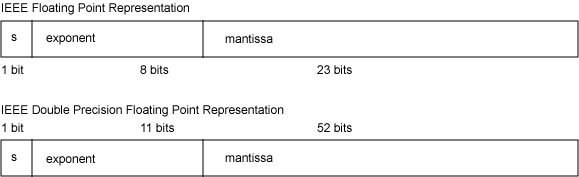
\includegraphics[width=0.7\textwidth]{float_representation}

  \bigskip

  \begin{itemize}
  \item Floating-point number representation from left to right
    \begin{itemize}
    \item \alert{sign} ($s$, 1 bit, $0 \rightarrow -$, $1 \rightarrow +$)
    \item \alert{exponent} ($e$, 8 or 11 bit)
    \item \alert{significand} or \alert{mantissa} ($m$, 23 or 52 bit)
    \end{itemize}
  \item The exponent does not have a sign
    \begin{itemize}
    \item An exponent bias $b$ is subtracted from it (127 or 1023)
    \end{itemize}
  \item The significand MSB is assumed to be $1$, unless the exponent is 0
  \end{itemize}

  \begin{align}
    x = s \times m \times 2^{e - b}
  \end{align}
\end{frame}


\begin{frame}[fragile]
  \frametitle{A simple example}
  \framesubtitle{\url{https://babbage.cs.qc.cuny.edu/IEEE-754/index.xhtml}}
  \begin{itemize}
  \item Take a floating-point number with an exact binary representation
  \end{itemize}
  \begin{align}
    0.75_{10} = 0.11_{2} = 0 \times 2 + 1 \times 2^{-1} + 1 \times 2^{-2} =
    \frac{1}{2} + \frac{1}{4} = 1.5 \times 2^{-1}
  \end{align}

  \begin{Verbatim}
0.75 -> 0x3F400000 = 0b|0|01111110|10000000000000000000000
sign = 0b0 = 0 -> +
exponent = 0b01111110 = 126 -> 126 - 127 = -1
significand = 0b(1)10000000000000000000000 = 12582912 -> 0b1.1 = 1.5
  \end{Verbatim}
  \begin{itemize}
  \item The representation of any floating point number is equivalent to the
    ratio of two integers, where the denominator is a power of 2
  \end{itemize}

  \begin{align}
    x = \frac{m}{2^{23 - e}} = \frac{12582912}{2^{24}} = \frac{3}{4} = 0.75
  \end{align}
\end{frame}


\begin{frame}[fragile]
  \frametitle{Floating point representation in Python}
  \begin{Verbatim}[label=\makebox{\url{https://bitbucket.org/lbaldini/programming/src/tip/snippets/float.py}},commandchars=\\\{\}]
\PY{n}{a} \PY{o}{=} \PY{l+m+mf}{0.75}
\PY{n}{num}\PY{p}{,} \PY{n}{den} \PY{o}{=} \PY{n}{a}\PY{o}{.}\PY{n}{as\PYZus{}integer\PYZus{}ratio}\PY{p}{(}\PY{p}{)}
\PY{k}{print}\PY{p}{(}\PY{n}{num}\PY{p}{,} \PY{n}{den}\PY{p}{)}
\PY{k}{print}\PY{p}{(}\PY{l+s+s1}{\PYZsq{}}\PY{l+s+s1}{\PYZob{}:.30f\PYZcb{}}\PY{l+s+s1}{\PYZsq{}}\PY{o}{.}\PY{n}{format}\PY{p}{(}\PY{n}{num} \PY{o}{/} \PY{n}{den}\PY{p}{)}\PY{p}{)}

\PY{k}{print}\PY{p}{(}\PY{p}{)}

\PY{n}{b} \PY{o}{=} \PY{l+m+mf}{0.1}
\PY{n}{num}\PY{p}{,} \PY{n}{den} \PY{o}{=} \PY{n}{b}\PY{o}{.}\PY{n}{as\PYZus{}integer\PYZus{}ratio}\PY{p}{(}\PY{p}{)}
\PY{k}{print}\PY{p}{(}\PY{n}{num}\PY{p}{,} \PY{n}{den}\PY{p}{)}
\PY{k}{print}\PY{p}{(}\PY{l+s+s1}{\PYZsq{}}\PY{l+s+s1}{\PYZob{}:.30f\PYZcb{}}\PY{l+s+s1}{\PYZsq{}}\PY{o}{.}\PY{n}{format}\PY{p}{(}\PY{n}{num} \PY{o}{/} \PY{n}{den}\PY{p}{)}\PY{p}{)}

[Output]
3 4
0.750000000000000000000000000000

3602879701896397 36028797018963968
0.100000000000000005551115123126
\end{Verbatim}

  \begin{itemize}
  \item as\_integer\_ratio() returns the internal representation of a float
  \item Mind this is not guaranteed to be the closest rational approximation
  \end{itemize}
\end{frame}


\begin{frame}
  \frametitle{Floating point representation}
  \framesubtitle{IEEE 754 standard}
  \begin{itemize}
  \item Good properties:
    \begin{itemize}
    \item numbers at wildly different magnitudes
    \item same relative accuracy at all magnitudes
    \item allow calculations across magnitudes
    \end{itemize}
  \item Dynamic range dictated by the number $n_e$ of bits in the exponent
    \begin{itemize}
    \item[] Range: $2^{2^{n_e - 1}}$
    \end{itemize}
  \item Precision dictated by the number $n_s$ of bits in the significand
    \begin{itemize}
    \item[] Precision: $log_{10} (2^{n_s + 1})$
    \end{itemize}
  \end{itemize}

  \bigskip

  \centering\begin{tabular}{llll}
    \hline
    Precision & Bits & Dynamic range & Digits of precision\\
    \hline
    \hline
    Single & $1 + 8 + 23 = 32$ & $\approx 2^{128} \text{ or } 10^{38}$ &
    7 \\
    Double & $1 + 11 + 52 = 64$ & $\approx 2^{1024} \text{ or } 10^{308}$ &
    15 \\
    \hline
  \end{tabular}
\end{frame}


\begin{frame}
  \frametitle{References}
  \scriptsize
  \begin{itemize}
  \item\url{https://scipy-lectures.org/}
  \item\url{https://docs.quantifiedcode.com/python-anti-patterns/}
  \item\url{https://sebastianraschka.com/Articles/2014_python_2_3_key_diff.html}
  \item\url{https://www.python.org/dev/peps/pep-0020/}
  \item\url{https://www.python.org/dev/peps/pep-0008/}
  \item\url{https://docs.python-guide.org/writing/style/}
  \item\url{https://docs.python.org/3/library/stdtypes.html}
  \item\url{https://docs.python.org/3/tutorial/controlflow.html\#defining-functions}
  \item\url{https://docs.python.org/3/tutorial/floatingpoint.html}
  \item\url{https://floating-point-gui.de/}
  \item\url{https://www.itu.dk/~sestoft/bachelor/IEEE754_article.pdf}
  \end{itemize}
\end{frame}



\end{document}
